\documentclass[12pt]{article}
% Math Packages
\usepackage{amssymb, amsmath, amsfonts, amsthm, mathtools, graphicx, tcolorbox, cancel, mathrsfs}

% Formatting Packages
\usepackage{cite, pdfpages, tikz, pgffor, float, pgfplots, import, xcolor, transparent, siunitx, caption, enumitem, titlesec, multicol, pifont, verbatim, fancyvrb, calc, xspace}


\usepackage{wrapfig,paralist,rotating,subfig}
\usepackage[textwidth=6in,textheight=8in]{geometry}

% Please use vector graphics in .pdf format where possible
% This is much preferable to large bitmap files
\DeclareGraphicsExtensions{{.pdf},{.jpg},{.png}}

\usepackage[english]{babel}
% \usepackage[utf8]{inputenc}
\usepackage[dvipsnames]{xcolor}
\usepackage[absolute]{textpos}

\usepackage{blindtext}


\usetikzlibrary{shapes.geometric}
\pgfplotsset{compat=1.18}
\pdfsuppresswarningpagegroup=1
\tikzset{every picture/.style={line width=0.75pt}}

\renewcommand{\baselinestretch}{1.5}

\newcommand{\eref}[2][]{%
	\ifthenelse{\equal{#1}{}}%
	{Eq.~(\ref{eq:#2})}%
	{Equation~(\ref{eq:#2})}\xspace}

% To refer to a figure, use \fref{<label>}, where <label> is the
% part that follows the 'fig:' in the label of the figure.
\newcommand{\fref}[2][]{%
  \ifthenelse{\equal{#1}{}}%
	{Fig.~\ref{fig:#2}}%
	{Figure~\ref{fig:#2}}}

% How to type vectors. If you don't like this style, you can just change
% the definition of \VEC!!
\newcommand{\VEC}[1]{\ensuremath{\boldsymbol{#1}}\xspace}

% unit vectors
\newcommand{\ux}{\ensuremath{\mathbf{\hat{x}}}\xspace}
\newcommand{\uy}{\ensuremath{\mathbf{\hat{x}}}\xspace}
\newcommand{\uz}{\ensuremath{\mathbf{\hat{x}}}\xspace}

% theta dot and double dot
\newcommand{\thd}{\ensuremath{\dot{\theta}}\xspace}
\newcommand{\thdd}{\ensuremath{\ddot{\theta}}\xspace}

% Derivatives. Some publications require the d in a differential
% to be set in roman. I've never liked that, but I have trained myself
% always to use these two macros, so if I need to switch, it is
% painless.
\newcommand{\DD}{\ensuremath{d}}		% differential d without leading space
\newcommand{\dd}{\ensuremath{\,\DD}}	% differential d

% A normal (total) derivative. If you supply an optional argument n,
% then you get the nth derivative: e.g., \deriv[2]{x}{t}
\newcommand{\deriv}[3][]{\ensuremath{%
	\ifthenelse{\equal{#1}{}}{\frac{\DD #2}{\DD #3}}
	{\frac{\DD^{#1} #2}{\DD #3^{#1}}}}}

% partial derivative
\newcommand{\pd}[3][]{\ensuremath{%
	\ifthenelse{\equal{#1}{}}{\frac{\partial #2}{\partial #3}}
	{\partial #2 / \partial #3}}}

% variational derivative
\newcommand{\varder}[2][]{\ensuremath{\deriv{}{t} \left( \pd{L}{\dot{#2}%
      \ifthenelse{\equal{}{#1}}{}{_{#1}}} \right)} - \pd{L}{#2%
      \ifthenelse{\equal{}{#1}}{}{_{#1}}} }

% variational derivative
\newcommand{\ele}[2][]{\ensuremath{\deriv{}{t} \left( \pd{\mathscr{L}}{\dot{#2}%
      \ifthenelse{\equal{}{#1}}{}{_{#1}}} \right)} = \pd{\mathscr{L}}{#2%
      \ifthenelse{\equal{}{#1}}{}{_{#1}}} }


\titlespacing\section{0pt}{12pt plus 4pt minus 2pt}{0pt plus 2pt minus 2pt}

\title{Phys 111 Computational Project}
\author{Aidan Gallade, Jonathan Holcombe}

\begin{document}
\maketitle

\section{Introduction}
Our chosen system consists of two charged particles, with charges $q_{1}$ and $q_{2}$  and masses $m_{1}$ and $m_{2}$ respectively, placed in a constant magnetic field, for simplicity's sake chosen to be $\mathbf{B} = B_{0}\, \hat{z}$.

In a system with just a single charged particle and a constant magnetic field along $\hat{z}$, the particle undergoes gyration in the $x$-$y$ plane about an axis parallel to $\hat{z}$ and approaches some constant speed in the $\hat{z}$ direction, as depicted in \fref{single-gyration}. If we take $|q|=|m| = 1$, then this terminal $z$-velocity is determined by $B_{0}$, and the radius of gyration is determined by both $B_{0}$ and the particle's initial velocity in the $x$-$y$ plane.

\begin{figure}[H]
    \centering
    \scalebox{1.4}{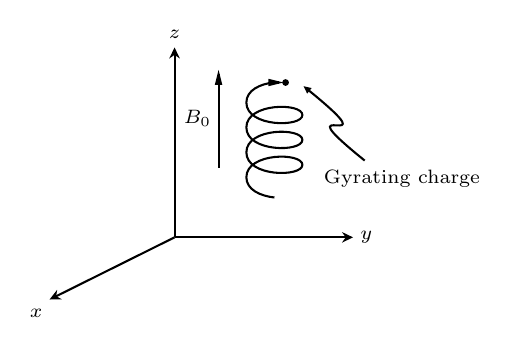
\begin{tikzpicture}[x=0.75pt,y=0.75pt,yscale=-1,xscale=1]
%uncomment if require: \path (0,300); %set diagram left start at 0, and has height of 300

%Straight Lines [id:da5273852527288051] 
\draw    (80.4,109.6) -- (80.4,21.1) ;
\draw [shift={(80.4,18.1)}, rotate = 90] [fill={rgb, 255:red, 0; green, 0; blue, 0 }  ][line width=0.08]  [draw opacity=0] (5.36,-2.57) -- (0,0) -- (5.36,2.57) -- (3.56,0) -- cycle    ;
%Straight Lines [id:da739028329510433] 
\draw    (80.4,109.6) -- (163.4,109.6) ;
\draw [shift={(166.4,109.6)}, rotate = 180] [fill={rgb, 255:red, 0; green, 0; blue, 0 }  ][line width=0.08]  [draw opacity=0] (5.36,-2.57) -- (0,0) -- (5.36,2.57) -- (3.56,0) -- cycle    ;
%Straight Lines [id:da657069656246055] 
\draw    (80.4,109.6) -- (22.87,138.22) ;
\draw [shift={(20.18,139.55)}, rotate = 333.55] [fill={rgb, 255:red, 0; green, 0; blue, 0 }  ][line width=0.08]  [draw opacity=0] (5.36,-2.57) -- (0,0) -- (5.36,2.57) -- (3.56,0) -- cycle    ;
%Straight Lines [id:da03660729578880251] 
\draw    (101.6,76) -- (101.6,30.92) ;
\draw [shift={(101.6,28.92)}, rotate = 90] [fill={rgb, 255:red, 0; green, 0; blue, 0 }  ][line width=0.08]  [draw opacity=0] (7.2,-1.8) -- (0,0) -- (7.2,1.8) -- cycle    ;
%Shape: Spring [id:dp1109537082947083] 
\draw   (128.5,90.4) .. controls (121.75,89.65) and (115,86.65) .. (115,80.65) .. controls (115,68.65) and (142,68.65) .. (142,74.65) .. controls (142,80.65) and (115,80.65) .. (115,68.65) .. controls (115,56.65) and (142,56.65) .. (142,62.65) .. controls (142,68.65) and (115,68.65) .. (115,56.65) .. controls (115,44.65) and (142,44.65) .. (142,50.65) .. controls (142,56.65) and (115,56.65) .. (115,44.65) .. controls (115,38.7) and (121.63,35.7) .. (128.32,34.92) ;
%Straight Lines [id:da009357086831838335] 
\draw    (129.84,35) -- (130.8,35) ;
\draw [shift={(132.8,35)}, rotate = 180] [fill={rgb, 255:red, 0; green, 0; blue, 0 }  ][line width=0.08]  [draw opacity=0] (7.2,-1.8) -- (0,0) -- (7.2,1.8) -- cycle    ;
%Shape: Circle [id:dp16217087388996976] 
\draw  [fill={rgb, 255:red, 0; green, 0; blue, 0 }  ,fill opacity=1 ] (132.8,35) .. controls (132.8,34.4) and (133.29,33.91) .. (133.89,33.91) .. controls (134.49,33.91) and (134.98,34.4) .. (134.98,35) .. controls (134.98,35.6) and (134.49,36.09) .. (133.89,36.09) .. controls (133.29,36.09) and (132.8,35.6) .. (132.8,35) -- cycle ;
%Curve Lines [id:da03245436193053908] 
\draw    (172,72.6) .. controls (128.84,37.71) and (187.96,73.67) .. (144.63,38.44) ;
\draw [shift={(142.58,36.78)}, rotate = 38.84] [fill={rgb, 255:red, 0; green, 0; blue, 0 }  ][line width=0.08]  [draw opacity=0] (3.57,-1.72) -- (0,0) -- (3.57,1.72) -- cycle    ;

% Text Node
\draw (18.18,142.55) node [anchor=north east] [inner sep=0.75pt]  [font=\scriptsize] [align=left] {$\displaystyle x$};
% Text Node
\draw (168.4,109.6) node [anchor=west] [inner sep=0.75pt]  [font=\scriptsize] [align=left] {$\displaystyle y$};
% Text Node
\draw (80.4,15.1) node [anchor=south] [inner sep=0.75pt]  [font=\scriptsize] [align=left] {$\displaystyle z$};
% Text Node
\draw (99.6,52.46) node [anchor=east] [inner sep=0.75pt]  [font=\scriptsize] [align=left] {$\displaystyle B_{0}$};
% Text Node
\draw (190,75.6) node [anchor=north] [inner sep=0.75pt]  [font=\scriptsize] [align=left] {Gyrating charge};


    \end{tikzpicture}}
    \caption{A single charge gyrating in the uniform static magnetic field $\mathbf{B} = B_{0}\, \hat{z}$.}
    \label{fig:single-gyration}
\end{figure}

By introducing a second particle, there will now be a Coulombic interaction between the two particles in addition to the circulating force felt from the magnetic field. Due to the Coulomb potential being proportional to $1/r$, we hope to see strong sensitivity to initial conditions and chaotic behavior as a result of introducing this second particle.

\section{Equations of Motion}
\subsection{Generalized Coordinates}
Since our system consists of two particles in three dimensions, this system has a maximum of six degrees of freedom. If we made certain assumptions about the mass or charge of the particle (such as the particles having equal charge-mass ratios), we might be able to reduce the number of degrees of freedom, but since we are not making any of these assumption, we are left with the initial six degrees of freedom, with generalized coordinates given by:
\[
(x_{1},y_{1},z_{1})\quad  (x_{2},y_{2},z_{2}).
\]

\subsection{Lagrangian(s)}
The Lagrangian of a single point charge $q$ in an electric and magnetic field is given by
\begin{align}
    \mathscr{L}(\mathbf{r},t) = \frac{1}{2}m \dot{\mathbf{r}}^{2} - q\, \phi(\mathbf{r},t) + q \,\dot{\mathbf{r}} \cdot \mathbf{A}(\mathbf{r},t) \label{eq:L_gen}
\end{align}
where $\phi(\mathbf{r},t)$ is the scalar potential of the electric field and $\mathbf{A}(\mathbf{r},t)$ is the vector potential of the magnetic field. Our system has a constant magnetic field of strength $B_{0}$ in the $\hat{z}$ direction, which has a vector potential of 
\begin{align}
    \mathbf{A}(\mathbf{r},t) = \mathbf{A} = -B_{0}y\;\hat{x}.
\end{align}
Since we have only two charged particles, the only electric field felt by one particle is the electric field of other particle, so the electric scalar potential of each particle is given by
\begin{align}
    \phi_{i}(\mathbf{r},t) = \frac{1}{4\pi\epsilon_{0}} \frac{q_{j}}{|\mathbf{r}_{i} - \mathbf{r}_{j}|} = \frac{1}{4\pi\epsilon_{0}} \frac{q_{j}}{d}
\end{align}
where we have defined $d = |\mathbf{r}_{i} - \mathbf{r}_{j}|$.

Substituting these potentials and our generalized coordinates into \eref{L_gen}, we get the Lagrangians of our two particles:
\begin{subequations}
    \label{eq:L}
    \begin{align}
    \mathscr{L}_{1}(x_{1},y_{1},z_{1}) = \frac{1}{2}m_{1} (\dot{x}_{1}^{2} + \dot{y}_{1}^{2} + \dot{z}_{1}^{2}) - \frac{1}{4\pi\epsilon_{0}} \frac{q_{1}q_{2}}{d} - q_{1}B_{0}y_{1}\dot{x}_{1}, \label{eq:L1} \\ 
    \mathscr{L}_{2}(x_{2},y_{2},z_{2}) = \frac{1}{2}m_{2} \dot(\dot{x}_{2}^{2} + \dot{y}_{2}^{2} + \dot{z}_{2}^{2}) - \frac{1}{4\pi\epsilon_{0}} \frac{q_{2}q_{1}}{d} - q_{2}B_{0}y_{2}\dot{x}_{2}, \label{eq:L2}
\end{align}
\end{subequations}
where $d$ is given by $\sqrt{(x_{2}-x_{1})^{2} +(y_{2}-y_{1})^{2} + (z_{2}-z_{1})^{2}  }$.

\subsection{Euler-Lagrange Equations}
Taking the Euler-Lagrange equations of these two Lagrangians, we get the following six differential equations:
\begin{subequations}
    \label{eq:ele1}
    \begin{align}
    \ele[1]{x}\implies&\ddot{x}_{1}=\frac{q_{1}B_{0}}{m_{1}}\dot{y}_{1}+\frac{q_{1}q_{2}}{4\pi \varepsilon_{0}m_{1}}\frac{x_{2}-x_{1}}{d^{3} }  \label{eq:elex1}   \\
    \ele[1]{y}\implies&\ddot{y}_{1}=-\frac{q_{1}B_{0}}{m_{1}}\dot{x}_{1} +\frac{q_{1}q_{2}}{4\pi \varepsilon_{0}m_{1}}\frac{y_{2}-y_{1}}{d^{3} }   \label{eq:eley1}       \\
    \ele[1]{z}\implies&\ddot{z}_{1} = \frac{q_{1}q_{2}}{4\pi \varepsilon_{0}m_{1}}\frac{z_{2}-z_{1}}{d^{3} } \label{eq:elez1} 
\end{align}
\end{subequations}
\begin{subequations}
    \label{eq:ele2}
    \begin{align}
    \ele[2]{x}\implies&\ddot{x}_{2}=\frac{q_{2}B_{0}}{m_{2}}\dot{y}_{2}-\frac{q_{1}q_{2}}{4\pi \varepsilon_{0}m_{2}}\frac{x_{2}-x_{1}}{d^{3} }   \label{eq:elex2}  \\
    \ele[2]{y}\implies&\ddot{y}_{2}=-\frac{q_{2}B_{0}}{m_{2}}\dot{x}_{2} -\frac{q_{1}q_{2}}{4\pi \varepsilon_{0}m_{2}}\frac{y_{2}-y_{1}}{d^{3} }    \label{eq:eley2}      \\
    \ele[2]{z}\implies&\ddot{z}_{2} = -\frac{q_{1}q_{2}}{4\pi \varepsilon_{0}m_{2}}\frac{z_{2}-z_{1}}{d^{3} }\label{eq:elez2}
\end{align}
\end{subequations}


\subsection{Non-dimensionalization}
To non-dimensionalize our equations of motion, we can combine the constants we have in our equations (e.g., $q,m,\varepsilon_{0},B_{0}$) to construct non-dimensionalized lengths and time:
\[
\left[ \left( \frac{B_{0}^2\varepsilon_{0}}{m} \right)^{1/3}   \right]  = \mathrm{m}^{-1} \qquad \left[ \frac{qB_{0}}{m} \right] = \mathrm{s}^{-1}. 
\]
Using these to write our generalized coordinates and their derivatives in terms of dimensionless variables, we get
\[
t = \tilde{t}\frac{m}{qB_{0}}, \qquad l = \tilde{l}\left(\frac{m}{B_{0}^2\varepsilon_{0}} \right)^{1/3}\hspace{-12pt},
\]
\[
\frac{dl }{dt }= \left( \frac{qB_{0}}{m} \right)\left( \frac{m}{B_{0}^2\varepsilon_{0}}   \right) ^{1/3}\frac{d^{2}\tilde{l} }{d\tilde{t}^{2} }, \qquad \frac{dl^{2} }{dt^{2} }= \left( \frac{qB_{0}}{m} \right)^{2}\left( \frac{m}{B_{0}^2\varepsilon_{0}}   \right) ^{1/3}\frac{d^{2}\tilde{l} }{d\tilde{t}^{2} }
\]
where $l$ is some generalized coordinate with units of length (e.g. $x$, $y$, or $z$).

For simplicity, we pick $q_{1}$ and $m_{1}$ to replace the $q$ and $m$ in these constants (picking $q_{2}$ and $m_{2}$ would be equally valid, but we need to be consistent). Substituting these non-dimensional variables into our equations of motion in \eref{ele1} and \eref{ele2}, we arrive at 
\begin{subequations}
\begin{align}
    &  \ddot{\tilde{x}}_{1} = \dot{\tilde{y}}  - \frac{1}{4\pi} \frac{q_{2} }{ q_{1}} \frac{\tilde{x}_{2}-\tilde{x}_{1}}{\tilde{d}^{3} }     \tag{7a}\\
    &  \ddot{\tilde{y}}_{1} = -\dot{\tilde{x}}  - \frac{1}{4\pi}\frac{q_{2} }{q_{1}} \frac{\tilde{y}_{2}-\tilde{y}_{1}}{\tilde{d}^{3} }          \tag{7b}\\
    &  \ddot{\tilde{z}}_{1} = -\frac{1}{4\pi}\frac{q_{2} }{q_{1}} \frac{\tilde{z}_{2}-\tilde{z}_{1}}{\tilde{d}^{3} }   \tag{7c}\\
    &  \ddot{\tilde{x}}_{2}=\frac{q_{2}m_{1}}{q_{1}m_{2}}\dot{\tilde{y}}_{2}+ \frac{1}{4\pi}\frac{q_{2}m_{1}}{ q_{1}m_{2}}\frac{\tilde{x}_{2}-\tilde{x}_{1}}{\tilde{d}^{3} }    \tag{8a}\\
    &  \ddot{\tilde{y}}_{2}=-\frac{q_{2}m_{1}}{q_{1}m_{2}}\dot{\tilde{x}}_{2}+ \frac{1}{4\pi}\frac{q_{2}m_{1}}{ q_{1}m_{2}}\frac{\tilde{y}_{2}-\tilde{y }_{1}}{\tilde{d}^{3} }          \tag{8b}\\
    &  \ddot{\tilde{z}}_{2} = \frac{1}{4\pi}\frac{q_{2}m_{1}}{ q_{1}m_{2}}\frac{\tilde{z}_{2}-\tilde{z}_{1}}{\tilde{d}^{3} } \tag{8c}
\end{align}
\end{subequations}
These $q$ and $m$ factor on our equations for the second particle just specify its behavior differs first particle's in terms of their charge and mass ratios.

\section{Dynamics}

Due to this system have twelve parameters for each initial condition ($x$, $y$, and $z$ for both particles and all of their first derivatives) in addition to the two charges $q_{1}$ and $q_{2}$ and the masses $m_{1}$ and $m_{2}$, the dynamics of this system are incredibly complex, and what counts as ``chaotic'' vs. ``non-chaotic'' isn't always clear\footnote[1]{Note than we will say something is ``chaotic" when nearby initial conditions have wildly different end results through iteration time along a reasonable timescale---the mathematical definition of chaos. We feel the need to mention this because a lot of what goes on in this system ``looks chaotic" (as is the colloquial definition of chaotic). When something ``looks chaotic," usually people mean that it is complicated and difficult to decipher. We will use the term ``funky" for describing mathematically non-chaotic behavior whose trajectories are complicated and difficult to decipher.}. 

To simplify our analysis, we set $m_{1}=m_{2}=1$ and $|q_{1}| = |q_{2}| = 1$, but do consider the situations of like charges and opposite charges. In our analysis of each of these situations, we consider the two cases of the particles starting from rest and starting with some initial velocity (in addition to all of the variation of initial conditions in each of those subcases). Furthermore, we let the particles pass through each other, should their trajectories take them on such a path.

This is in no way an exhaustive list of dynamics of this system. There are likely many more intricate behaviors this system is able to display that this higher-level description does not capture.

\subsection{Like Charges}
\subsubsection{No initial velocities ($\vec{v}_{0,i} = 0$)}

This setup exhibits no chaotic motion ever. With the exception of the clover pattern island when $z_{0}=0$ for both particles (explained below), all simulations here will end up with two particles gyrating away from each other for all eternity (\fref{like_repel_forever}). This is because their z-directional repulsion and subsequent z-velocity (which the B-field does not alter the direction of) will carry them away from each other. The gyration's shape is always a circle, and its size is dependent on the charge ratio or initial velocity. The travel speed (therefore the compactness of the gyration's coiling) is dependent on the mass ratio. Since we always keep both ratios at 1, any changes in the gyration radius or coil compactness will be because of initial velocities. 

\begin{figure}[H]
    \centering
    \includegraphics[width=0.6\linewidth]{figures/like_zero_away.png}
    \caption{The usual steady state for repulsive particles with no initial velocities. Don't be fooled into thinking the gyration is elliptical here---the $x$- and $y$-aspect ratios are different.}
    \label{fig:like_repel_forever}
\end{figure}

A subset of these conditions is when they have the same $x$- and $y$-coordinates too, in which they will not gyrate at all and will simply repel each other perfectly Coulombically. %(Examples of different radii and different coil compactness will be shown later.)

If the particles both have the same $z$-coordinate but different $x$- and $y$-coordinates, they will form a funky clover pattern (as shown  in \fref{clover})---a repeating cycle where they repel each other near their common center, then arc around (due to the magnetic field curving their $x$-$y$ velocities) to meet each other again at some new angle around the circle (basically a new precession angle, similar to Mercury's orbit), repeating indefinitely. The closer they are to each other to begin with, the stronger their initial repulsion, so the more complete a circle they form, and the smaller the precession angle per cycle (\fref{clover_small}). However, if the precession angle's ratio with $2\pi$ happens to be a rational number, then it will take much longer, and we get flowers (\fref{clover_ratio}).


\begin{figure}[H]
    \centering
    \begin{subfigure}[t]{0.45\textwidth}
        \centering
        \includegraphics[height=2.6in]{figures/clover_pattern.png}
        \caption{An example of a clover pattern.}
        \label{fig:clover}      
    \end{subfigure}
    \begin{subfigure}[t]{0.45\textwidth}
        \centering
        \includegraphics[height=2.6in]{figures/clover_small_precession.png}
        \caption{A clover with a small precession angle, iterated for only a few circulations. If we let the simulation run longer, it would form a thick magenta ring}
        \label{fig:clover_small}       
    \end{subfigure}
    \caption{Clover patterns of like charges with $\vec{v}=0$ and $z_{0} = 0$ precessing about their common center as they circulate due to the $B$ field.}
\end{figure}

\begin{figure}
      \centering
        \includegraphics[height=2.8in]{figures/clover_ratio_precession.png}
        \caption{A clover where the precession angle ratio happens to be near $2\pi / 5$, resulting in 5-pointed flowers.}
        \label{fig:clover_ratio}    
\end{figure}


\subsubsection{Non-zero initial velocities}
This setup still exhibits no chaotic motion ever. The coil compactness is dependent on the initial $z$-velocity---if it moves faster in $z$, it will coil less tightly. The gyration radius is dependent on the initial x- and $y$-velocities. The larger the velocities, the larger the gyration radius.

The two particles will rarely ever interact Coulombically in a way that meaningfully changes the system dynamics from the at-rest cases, since they will be pulled away from each other by the magnetic field quickly. However, the island of instability on which the clover pattern initial conditions live becomes a bit larger now, since, so long as there is no initial $z$-velocity, clover patterns of various proportions can form. The patterns may now be radially asymmetric (\fref{clover_asymmetric}) and, in general, even more funky-looking (\fref{clover_funky}).
\begin{figure}[H]
    \centering
    \begin{subfigure}[t]{0.45\textwidth}
        \centering
        \includegraphics[height=2.2in]{figures/asymmetric_clover.png}
        \caption{Radially asymmetric clover pattern, resulting from a large, asymmetric initial velocity in one direction. Looks more like a plum than a clover.}
        \label{fig:clover_asymmetric}      
    \end{subfigure}
    \begin{subfigure}[t]{0.45\textwidth}
        \centering
        \includegraphics[height=2.1in]{figures/funky_clover.png}
        \caption{A very funky clover.}
        \label{fig:clover_funky}      
    \end{subfigure}

    \caption{Clover patterns of like charges with $\vec{v}\ne0$ and $z_{0} = 0$.}
\end{figure}

\subsection{Opposite Charges}

\subsubsection{No initial velocities ($\vec{v}_{0,i} = 0$)}
When both particles only vary by a $z$-position, we have an unstable equilibrium where they oscillate up and down (since the particles are free to pass through each other). Varying from this by even a tiny bit results in chaotic motion.
\paragraph{Same $z$, Different $x$ and $y$:}
If the particles are very far apart, the Coulombic interaction cannot overpower the $B$-field wishing to curve their trajectories. Thus, they make semicircular arcs, traveling in one direction (determined by their initial offsets and their individual charge) in tandem for eternity (\fref{semi_arcs}) as a steady state.

\begin{figure}[H]
    \centering
    \includegraphics[width=0.5\linewidth]{figures/semi_arcs_small.png}
    \caption{The semi-circular arcs formed by the competing Coulomb and magnetic forces in the case where the $B$-field wins. The $B$-field moves the particles on a circular path (in opposite directions due to their opposite charge), aided by the Coulomb force. Once the $B$-field starts circulating them away from each other and overpowers the Coulomb force, it competes with the Coulomb force until the particles eventually come to rest, restarting the cycle.}
    \label{fig:semi_arcs}
\end{figure}


If the particles come very close together in their trajectories, the Coulombic interaction easily overpowers the $B$-field wishing to curve their trajectories. So, they careen towards each other, building speed. Eventually they pass each other, which causes them to slow down Coulombically, turn around, and then go back the other direction. Due to the $B$-field effects when they are moving faster, they then swing all the way back out to their initial starting-position-distance apart, but with some new sideways travel distance too (because of the minimal effect of the $B$-field) This process repeats indefinitely, again traveling in one direction in tandem for eternity (\fref{semi_arcs_coulomb}) as a steady state.

\begin{figure}[H]
    \centering
    \includegraphics[width=0.5\linewidth]{figures/semi_arcs_coulomb_wins.png}
    \caption{Trajectory where the Coulomb force (mostly) wins over $B$-field. Because these were initialized with an $x$-displacement, they travel towards the $+y$ direction in tandem. If they were initialized with a
    $y$-displacement, they would travel in the $-x$ direction.}
    \label{fig:semi_arcs_coulomb}
\end{figure}

There is a boundary condition when they are both initialized about 1.0838 to 1.0839 length-units apart. If their initial displacement is any greater than this length, the $B$-field wins and they are never allowed to cross paths (however the semicircles begin to resemble plateaus, as seen in \fref{semi_arcs_plateau}), but if it is any less, the Coulomb force wins and they are able to cross paths (but it is very brief, and they are quickly banished back to being far from one another). These paths looks like curly braces $\lbrace \;\rbrace$, as shown in \fref{semi_arcs_braces}. A phase-space plot of this latter case is shown in \fref{phase_space}.

\begin{figure}[H]
    \centering
    \begin{subfigure}[t]{0.4\textwidth}
        \centering
        \includegraphics[height=2.4in]{figures/semi_arcs_plateau.png}
        \caption{Boundary condition plateaus, with the\\$B$-field barely winning.}
        \label{fig:semi_arcs_plateau}
    \end{subfigure}\hspace{12pt}
    \begin{subfigure}[t]{0.4\textwidth}
        \centering
        \includegraphics[height=2.2in]{figures/semi_arcs_braces.png}
        \caption{Boundary condition braces, with the Coulomb force barely winning.}
        \label{fig:semi_arcs_braces}
    \end{subfigure}
    \caption{Trajectories on either side of the boundary condition.}
\end{figure}

\begin{figure}[H]
    \centering
    \begin{subfigure}[t]{0.8\textwidth}
        \captionsetup{labelformat=empty}
        \includegraphics[width=1\linewidth]{figures/poincare.png}
        \caption{Fig. 9a: Phase space plots of the curly-brace trajectory (full caption on next page).}
    \end{subfigure}\hspace{12pt} \\
\end{figure}

\addtocounter{figure}{-1}
\begin{figure}[H]
    \centering
    \begin{subfigure}[t]{0.75\textwidth}
        \centering
        \captionsetup{labelformat=empty}
        \includegraphics[width=0.8\linewidth]{figures/four_point.png}
        \caption{Fig. 9b: A zoomed out phase-space plot of $x_{1}$ and $\dot{x}_{1}$, showing the four-pointed star formed by the yellow trajectories.}
    \end{subfigure}\hspace{12pt}
    \caption{The first picture is of phase plots of various initial conditions extremely near to the boundary point. The deep purple graphs represent the cases where the $B$-field wins out, and the light yellow graphs represent the cases where the Coulomb force wins out. The travel direction was the $+y$ direction. Notice that the $B$-field winning means the graphs are constrained to a teardrop loop in the $x$-plots, while the Coulomb force winning means the graphs can extend beyond the teardrop. The resultant shape when the Coulomb force wins is a 4-pointed star with one of its points exhibiting the loop shown (the rightmost point, for this case), as demonstrated in the second picture. The aspect ratios make the two $x_{1}$ graphs seem different, but they are not: the yellow curves' $x_{1}$ graphs are the same shape as the second $x_{1}$ graph, but the second $x_{1}$ graph has the upper and lower star tips in view (and is therefore squished up-and-down)}
    \label{fig:phase_space}
\end{figure}

\paragraph{ Different $x$, $y$ and $z$.}
When all three of the particles' starting positions are different, we still get the same boundary condition of about 1.0838-1.0839 length-units apart causing a flip in which force win the war. Most behavior from the non-$z$-offset cases still apply here. However, there are some notable complications introduced by the z-directional oscillation:

When the Coulomb force wins easily, then the motion is very chaotic. There is Coulombic $z$-directional oscillation occurring alongside the funky oscillatory behavior described before, which combine to make very chaotic results (\fref{z_offset_c})

\begin{figure}[H]
    \centering
    \begin{subfigure}[t]{0.4\linewidth}
        \includegraphics[height=2in]{figures/z_offset_c_full.png}
    \end{subfigure}
     \begin{subfigure}[t]{0.4\linewidth}
        \includegraphics[height=2in]{figures/z_offset_c_top_down.png}
    \end{subfigure}
     \begin{subfigure}[t]{0.4\linewidth}
        \includegraphics[height=2in]{figures/z_offset_c_left.png}
    \end{subfigure}
    \caption{Chaotic behavior with initial $z$ offset of 0.5 and in which the Coulomb force wins easily.}
    \label{fig:z_offset_c}
\end{figure}


When the B-field wins easily, we see behavior extremely similar to the non-z-offset case, just with some z-directional oscillation added in (\fref{z_offset_b}).


\begin{figure}[H]
    \centering
    \begin{subfigure}[t]{0.4\linewidth}
        \includegraphics[height=2in]{figures/z_offset_b_full.png}
    \end{subfigure}
     \begin{subfigure}[t]{0.4\linewidth}
        \includegraphics[height=2in]{figures/z_offset_b_top_down.png}
    \end{subfigure}
     \begin{subfigure}[t]{0.4\linewidth}
        \includegraphics[height=2in]{figures/z_offset_b_left.png}
    \end{subfigure}
    \caption{Chaotic behavior with initial $z$ offset of 0.5 and in which the $B$-field wins easily.}
    \label{fig:z_offset_b}
\end{figure}


When initializing a condition very close to the boundary condition, we find that in some cycles the $B$-field wins and the particles don't come near each other. In other cycles, the Coulombic attraction wins and they do cross paths (as seen in \fref{z_offset}). This is because, near the boundary condition, it matters whether the $z$-offset oscillation and semicircular oscillation are in phase. If they are in phase, the particles draw near enough for Coulombic attraction to win. If they are out of phase, we do not get closer than the boundary length, and the $B$-field still ekes out a victory, preventing them from crossing paths. The phase plots in \fref{z_offset_phase} illustrate the phenomena well, especially compared to the non-$z$-offset case.

\begin{figure}[H]
    \centering
    \begin{subfigure}[t]{0.4\linewidth}
        \includegraphics[height=2in]{figures/z_offset_full.png}
    \end{subfigure}
     \begin{subfigure}[t]{0.4\linewidth}
        \includegraphics[height=2in]{figures/z_offset_top_down.png}
    \end{subfigure}
     \begin{subfigure}[t]{0.4\linewidth}
        \includegraphics[height=2in]{figures/z_offset_left.png}
    \end{subfigure}
    \begin{subfigure}[t]{0.4\linewidth}
        \includegraphics[height=2.2in]{figures/z_offset_pos.png}
    \end{subfigure}
    \caption{Example of a small (0.1) $z$-offset with initial distances very close to the boundary condition causing the war between B-field and Coulombic attraction to be indeterminate.The first graph is an angled view to show how non-uniform it is, and the second graph is an overhead view (since it is still a 3D render, there is some depth-of-view warping occurring). The third graph is a side-on view showing how the $z$-oscillation amplitudes are heavily modified by the other two forces. All of these effects (including the traveling) are very clear in the fourth graph (the position plots through time).}
    \label{fig:z_offset}
\end{figure}

\begin{figure}[H]
    \centering
    \includegraphics[width=0.7\linewidth]{figures/z_offset_phase.png}
    \caption{Phase plots of the small (0.1) z-offset with initial distances very close to the boundary condition. We have zoomed in on the $x_{1}$ graph, where it it more obvious that the teardrop-loop is completed in cycles where the $B$-field wins, and the teardrop loop is not completed (and the 4-pointed star is exhibited instead) in cycles where the Coulomb force wins. The $x_{1}$ and $x_2$ graphs look the same, except that they are both mirrored left-to-right, and $x_{2}$ is not zoomed-in like $x_{1}$ is.}
    \label{fig:z_offset_phase}
\end{figure}


\subsubsection{Non-zero Initial Velocities}
When both particles only vary by a $z$-position and $z$-velocity, we see no functional difference between this case and the from-rest unstable equilibrium. Beyond this, it becomes \textit{very} dynamically funky and chaotic. This could be the subject of a thesis given how much content there is to write about, so we will leave our discussion here.

\section{Conclusion}
To summarize this lengthy analysis, we first found that particles of opposite charge (and thus Coulombically repulsive) in a uniform static magnetic field exhibited no chaotic behavior. The particles either shot off to $z=+\infty$ and $z=-\infty$, circulating about $B_{0}$ the whole way, or oscillated about each other in clover-like patterns in the $x$-$y$ plane. 

The dynamics got much more interesting when we made the particles have opposite charges, and thus attractive. 

When the particles had no initial velocities but the same initial $z$-position, they traveled in a single direction (either $+y$ or $-x$) and oscillated in repeating pattern based on how close the particles came to each other. If they stayed far apart (i.e. the $B$-field won), they formed semi-circular arcs. If they got very close to each other (i.e. Coulomb force won), they overshot each other before being pulled back to either initial positions (plus some traveling offset). Between these two cases there was a boundary around $1.0838$ initial separation. Just above this distance, the $B$-field won and we saw plateau-shaped arcs, and just below, the Coulomb force won and we saw curly-brace-shaped arcs.

The truly chaotic behavior occurred when we had no initial velocities but differing $x$, $y$, and $z$ positions. Again, the behavior was dependent upon how close to the boundary condition (now at a slightly different distance) the particles got. When the $B$-field won, we saw behavior very similar to the same-initial-$z$ case, now with some non-trivial oscillation in the $z$-direction due to Coulombic interactions. When the Coulomb force won, the trajectories were almost entirely chaotic, beyond the high-level patterns of the trajectories crossing (since the Coulomb force overpowered the $B$-field) and some general oscillation in the $z$-direction. Near the boundary condition, whether the particles formed curly braces or plateaus depended on whether the $z$-oscillations of the particles were in phase or not, leading to semi-periodic cycles in which the particles only sometimes got close enough to overpower the $B$-field and form curly braces.


Due to the incredibly high-dimensional phase space of this system, we chose to do surface-level passes of each of the categories of initial conditions, rather exploring one particular category in depth. Future work could dive much deeper into the behavior of each of these categories of trajectories, including more quantitative analysis, such as where the boundary condition lies in a high-dimensional space (i.e. what is the ``boundary plane" as we increase the initial $z$ separation with opposite charge). Furthermore, we omitted analysis of opposite charges with non-zero initial velocity due to its complexity, so that is an additional area with many dynamical questions left to be explored.


\end{document}